\documentclass[conference]{IEEEtran}
\usepackage{graphicx}
\usepackage{booktabs}
\usepackage{amsmath,amssymb}
\usepackage{url}
\usepackage[hidelinks]{hyperref}
\title{Self-Supervised Memory-Bank Anomaly Detection for UAV Landing Pads: Whole-Pad versus Grid-Hybrid Representations under Synthetic Occlusions}
\author{\IEEEauthorblockN{Tolga Ferhan K\"u\c{c}\"uk}
\IEEEauthorblockA{Department of Computer Engineering\\
Kocaeli University, Kocaeli, T\"urkiye\\
\href{mailto:kucuktolgaferhan@gmail.com}{kucuktolgaferhan@gmail.com}\\
\url{https://github.com/tolgafk}}}
\begin{document}
\maketitle
\begin{abstract}
Autonomous landing requires rejection of pads affected by previously unseen objects or surface changes. This paper compares two nominal-only, self-supervised anomaly detectors for UAV landing areas. Zero-margin UAP/UAI regions are encoded by a ResNet-101 trained with a SimCLR objective, retained in a nominal memory bank, and scored by one minus maximum cosine similarity. Wholepad SSL embeds the complete region; Grid-Hybrid SSL splits it into a $2\times2$ grid and uses the maximum tile anomaly. Evaluation uses 630 clean test pads and 630 paired synthetic obstructions generated with randomized geometry, 22--65\% coverage, contrast-aware color, texture, contours, and shadows. Wholepad SSL achieves 0.9236 AUROC, 0.8583 F1, and 0.8563 accuracy. Grid-Hybrid SSL obtains 0.7555 AUROC and, at its stored threshold, 0.1667 F1 because recall falls to 0.0921. Threshold analysis improves the grid result but does not close the AUROC gap. The findings support whole-pad representation for the tested obstruction family while identifying calibration, feature dimensionality, and synthetic-to-real transfer as central limitations.
\end{abstract}
\begin{IEEEkeywords}
UAV, safe landing, anomaly detection, self-supervised learning, SimCLR, memory bank, synthetic occlusion
\end{IEEEkeywords}

\section{Introduction}
Reliable autonomous landing requires more than locating a designated pad. A vehicle must also reject a pad whose appearance has changed because of an unexpected object, surface damage, or partial occlusion. Supervised detectors such as YOLO are effective for known object categories, but their closed-set formulation does not directly cover every hazard that can occur after deployment~\cite{redmon2016,ruff2021}. This motivates a nominal-only formulation: learn the visual distribution of safe landing pads and flag inputs that depart from that distribution.

This work studies that formulation with two self-supervised representations. \emph{Wholepad SSL} embeds the complete pad region of interest (ROI). \emph{Grid-Hybrid SSL} divides the same ROI into a $2\times2$ grid, embeds each tile, and uses the most anomalous tile as the pad score. Both methods use contrastive representation learning, a memory bank of nominal embeddings, and nearest-neighbor cosine similarity. Their evaluation is intentionally focused on synthetically generated pad obstructions, because the available test split contains too few consistently labeled, real anomalous pads for a controlled comparison.

The contributions are threefold. First, a reproducible synthetic evaluation procedure creates geometrically and photometrically diverse pad occlusions while retaining paired clean controls. Second, global and tiled representations are compared under the same ROI and sample protocol. Third, the analysis separates threshold-free ranking quality from threshold-dependent operational behavior, exposing a large calibration sensitivity in the tiled model. On 630 clean and 630 paired synthetic samples, Wholepad SSL reaches 0.924 AUROC and 0.858 F1, whereas Grid-Hybrid SSL reaches 0.756 AUROC and 0.167 F1 at its stored operating threshold.

\section{Related Work}
Contrastive self-supervision learns invariances by bringing two augmented views of an image together while separating other instances. SimCLR operationalizes this idea with the normalized temperature-scaled cross-entropy (NT-Xent) loss~\cite{chen2020}. Contrastive objectives have also been adapted to novelty detection, where transformations and representation geometry help distinguish nominal data from shifted inputs~\cite{tack2020}. Recent surveys place such methods within a broader family of deep anomaly detectors that learn a description of normality rather than a closed set of abnormal classes~\cite{ruff2021,hojjati2022}.

Memory-bank methods retain nominal embeddings and score a query by its distance from nearby references. PatchCore demonstrates the value of pretrained patch representations and compact nominal memories for industrial anomaly detection~\cite{roth2022}; PaDiM models patch-level feature distributions~\cite{defard2021}; and deep pyramid correspondences show that sub-image matching can reveal local anomalies~\cite{cohen2020}. PANDA similarly adapts deep features for anomaly detection~\cite{reiss2021}. The present study adopts nearest-neighbor scoring but compares two ROI granularities for aerial landing pads. This setting differs from standard industrial benchmarks because pad scale, perspective, illumination, and surrounding context can vary substantially.

Visual safe-landing systems have long combined onboard vision with geometric or learned decision rules~\cite{yang2013}. More recent work studies safe landing-zone mapping in dynamic scenes~\cite{abdollahzadeh2026}, while DroneSSL applies self-supervision to multimodal anomaly detection in drone systems~\cite{akram2024}. Our scope is narrower: controlled synthetic obstruction generation and appearance-based anomaly detection inside labeled landing-pad ROIs.

\section{Method}
\begin{figure*}[t]
\centering
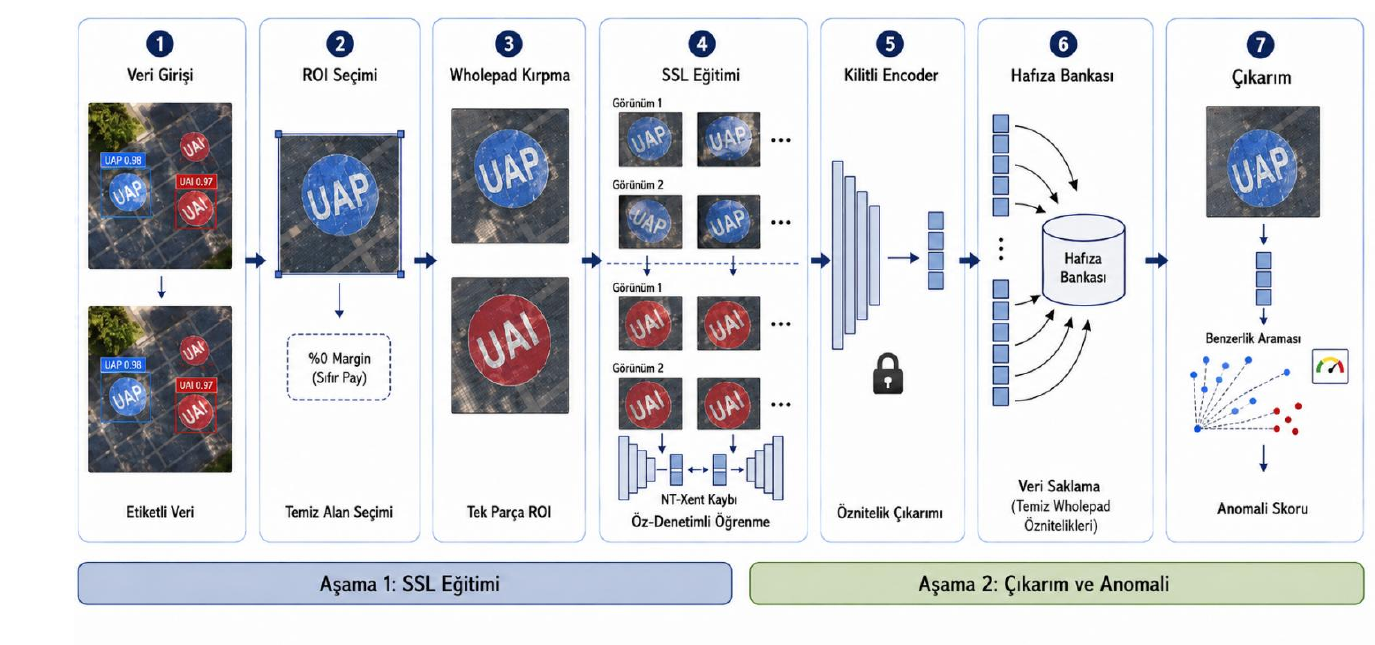
\includegraphics[width=0.96\textwidth]{figures/wholepad_workflow.png}
\caption{End-to-end Wholepad SSL workflow reproduced from the thesis: labeled input, zero-margin ROI selection, whole-pad contrastive learning, frozen encoding, nominal memory-bank construction, and cosine-similarity anomaly scoring.}
\label{fig:whole-workflow}
\end{figure*}

\begin{figure*}[t]
\centering
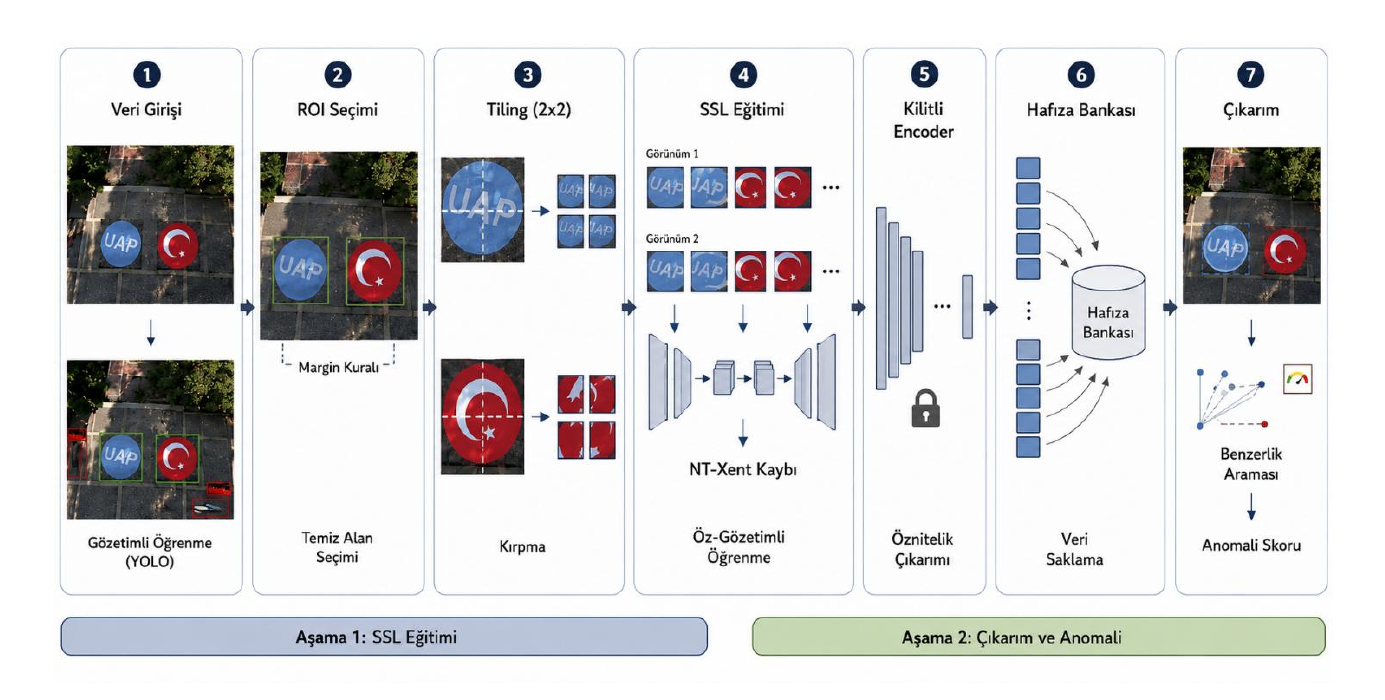
\includegraphics[width=0.96\textwidth]{figures/grid_workflow.png}
\caption{End-to-end Grid-Hybrid SSL workflow reproduced from the thesis. The landing-pad ROI is divided into a $2\times2$ grid before contrastive representation learning and memory-bank scoring.}
\label{fig:grid-workflow}
\end{figure*}

\subsection{ROI construction and nominal learning}
The complete processing paths are summarized in Figs.~\ref{fig:whole-workflow} and~\ref{fig:grid-workflow}. The source collection is the TEKNOFEST Aviation Artificial Intelligence data set, which contains more than 10,000 aerial images with YOLO-format annotations~\cite{teknofest2026}. Only the UAP and UAI landing-area classes are used to extract ROIs. Bounding boxes are converted from normalized coordinates to pixels and cropped with zero margin so that background texture outside the pad does not dominate the representation. ROIs smaller than 32 pixels in either dimension are discarded. All retained inputs are resized to $224\times224$ pixels.

A ResNet-101 encoder~\cite{he2016} is optimized on nominal pad crops with SimCLR. For a pad $x$, two stochastic augmentations $t_i$ and $t_j$ form a positive pair. Let $z_i$ and $z_j$ denote their normalized projected embeddings. The pairwise objective is
\begin{equation}
\ell_{i,j}=
-\log
\frac{\exp\!\left(\operatorname{sim}(z_i,z_j)/T\right)}
{\displaystyle\sum_{k=1}^{2N}\mathbb{1}_{[k\neq i]}
\exp\!\left(\operatorname{sim}(z_i,z_k)/T\right)},
\label{eq:ntxent}
\end{equation}
where $\operatorname{sim}$ is cosine similarity and $T=0.2$. Both implementations train for 20 epochs with AdamW, batch size 8, learning rate $3\times10^{-4}$, and random seed 42. The active experiment uses no supervised anomaly penalty; synthetic anomalies are introduced only for evaluation.

\subsection{Whole-pad and grid-hybrid representations}
Wholepad SSL preserves the complete zero-margin crop. The memory bank contains 5,968 L2-normalized, 2,048-dimensional encoder outputs. Given query embedding $z$ and nominal bank $\mathcal{B}$, its anomaly score is
\begin{equation}
A_{\mathrm{whole}}(x)
=1-\max_{b\in\mathcal{B}} z^{\top}b.
\label{eq:whole}
\end{equation}

Grid-Hybrid SSL divides each ROI into four fixed quadrants. Each tile is independently resized and encoded in the 128-dimensional projection space. The resulting bank contains 23,872 tile embeddings, exactly four times the whole-pad bank count. For tile embeddings $z_k$, $k\in\{1,\ldots,4\}$,
\begin{equation}
A_{\mathrm{grid}}(x)
=\max_{k\in\{1,\ldots,4\}}
\left[1-\max_{b\in\mathcal{B}_g}z_k^{\top}b\right].
\label{eq:grid}
\end{equation}
The query tile is compared with the pooled bank of all nominal tile positions. The final decision is
\begin{equation}
\widehat{y}(x)=
\begin{cases}
1\;(\textsc{unsafe}), & A(x)\geq\tau,\\
0\;(\textsc{safe}), & A(x)<\tau.
\end{cases}
\label{eq:decision}
\end{equation}
Wholepad uses a Youden-$J$ threshold of 0.01419 because no prior threshold was available. Grid-Hybrid uses the stored deployment threshold 0.1400. AUROC is reported independently of these operating points.

\subsection{Synthetic obstruction generation}
Each accepted clean test ROI produces a paired anomalous copy. A random target coverage between 22\% and 65\% of the ROI is sampled, followed by one of four masks: rotated rectangle, ellipse, band, or irregular eight-vertex polygon. Position, aspect ratio, and orientation are randomized. The fill color is selected from high-contrast candidates relative to the ROI median. Diagonal stripes, a contrasting contour, and an offset darkened shadow add internal texture and boundary cues. The generator therefore perturbs color, geometry, texture, and local illumination rather than applying a flat rectangular cutout.

The test scan covers 671 images and 650 annotated pad candidates. Twenty candidates are removed by the minimum-size rule, leaving 630 clean ROIs. Their paired synthetic copies yield a balanced set of 1,260 samples. Because each synthetic image is derived from its clean counterpart, the design controls pad identity but does not constitute an independent sample of real hazards.

\section{Results}
\begin{table*}[t]
\centering
\caption{Performance at the stored or fallback operating threshold. Positive denotes \textsc{unsafe}.}
\label{tab:main}
\small
\begin{tabular}{lrrrrrrrrr}
\toprule
Method & $\tau$ & AUROC & Precision & Recall & Specificity & F1 & Accuracy & TN/FP & FN/TP \\
\midrule
Wholepad SSL & 0.01419 & 0.9236 & 0.8470 & 0.8698 & 0.8429 & 0.8583 & 0.8563 & 531/99 & 82/548 \\
Grid-Hybrid SSL & 0.14000 & 0.7555 & 0.8788 & 0.0921 & 0.9873 & 0.1667 & 0.5397 & 622/8 & 572/58 \\
\bottomrule
\end{tabular}
\end{table*}

Table~\ref{tab:main} shows a 0.1681 absolute AUROC advantage for Wholepad SSL. Its operating point is also balanced: 548 of 630 synthetic anomalies are detected while 531 of 630 clean pads remain accepted. Grid-Hybrid produces only eight false alarms and consequently high precision, but misses 572 synthetic hazards. For a landing-safety gate, this false-negative concentration is more consequential than the low false-positive count.

\begin{figure*}[t]
\centering
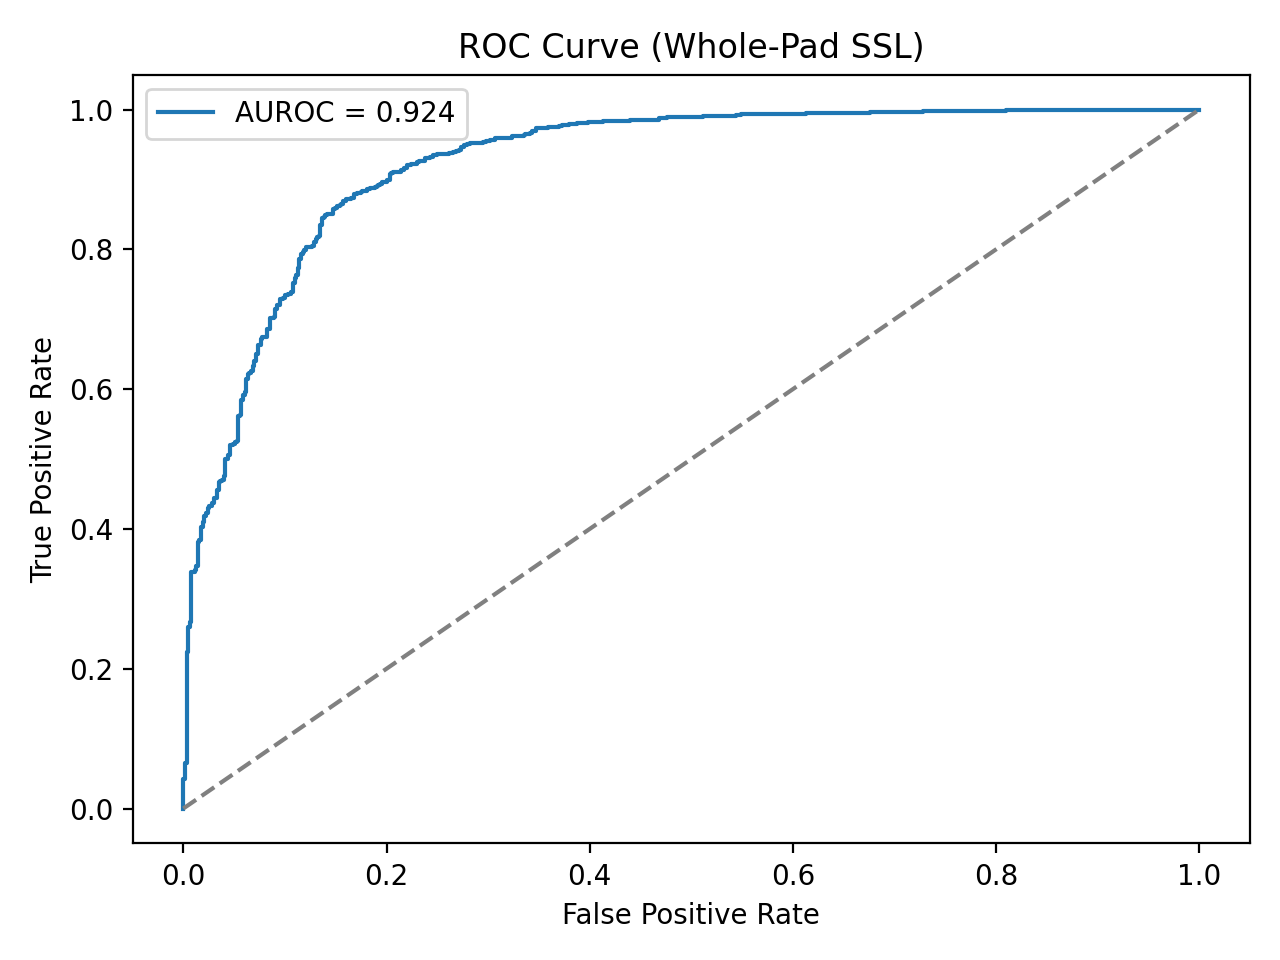
\includegraphics[width=0.47\textwidth]{figures/wholepad_roc.png}\hfill
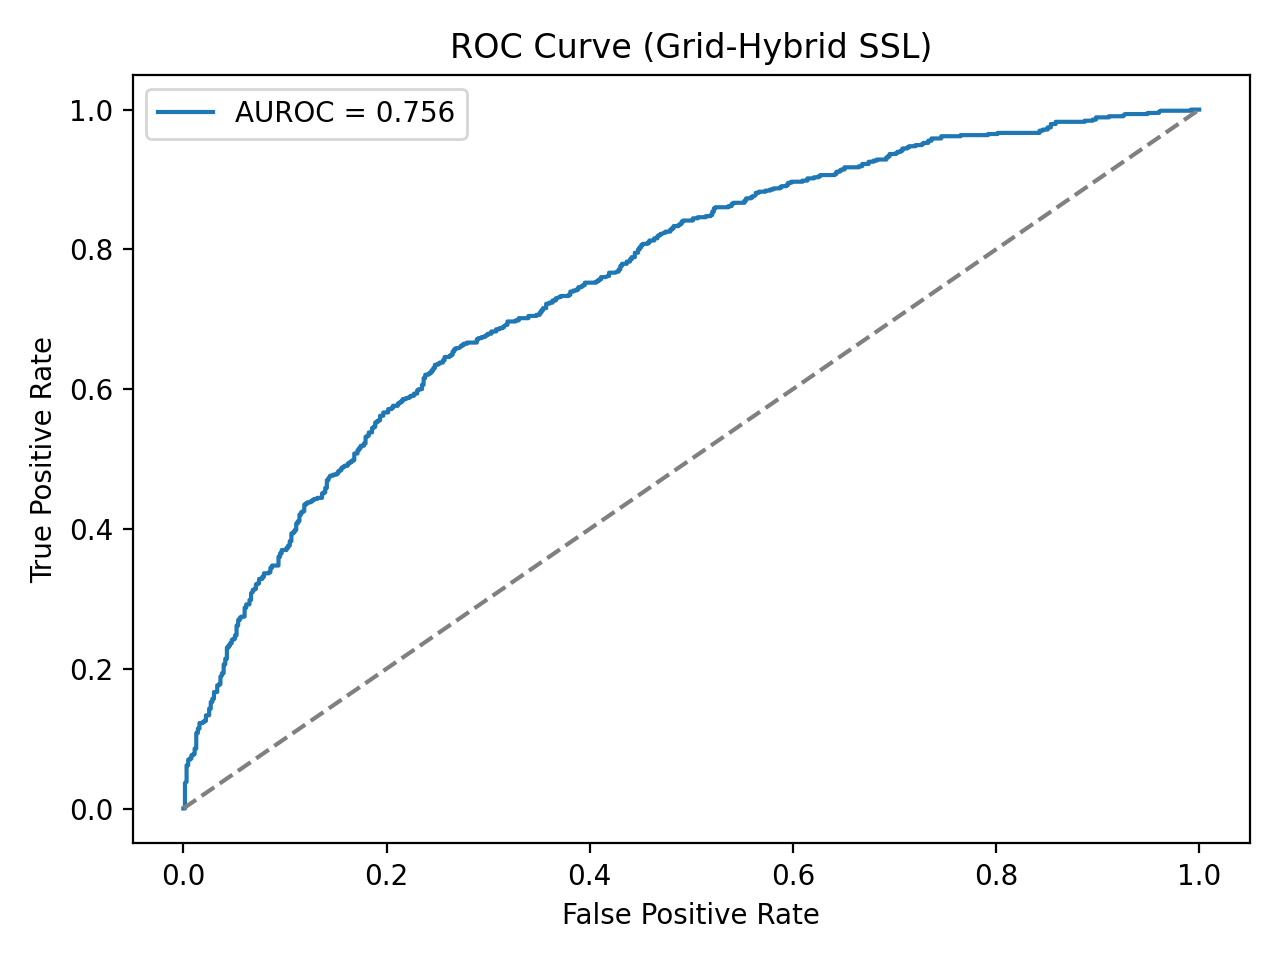
\includegraphics[width=0.47\textwidth]{figures/grid_roc.png}
\caption{Receiver operating characteristic curves for Wholepad SSL (left) and Grid-Hybrid SSL (right), evaluated on the same 630 clean and 630 synthetic samples.}
\label{fig:roc}
\end{figure*}

The ROC curves in Fig.~\ref{fig:roc} confirm that the conclusion is not solely a consequence of threshold selection. Wholepad ranks paired anomalies above clean pads more reliably across the full range of false-positive rates. Score histograms in Fig.~\ref{fig:hist} further show a clearer distribution shift for the global representation; Grid-Hybrid retains substantial overlap below its high stored threshold.

\begin{figure*}[t]
\centering
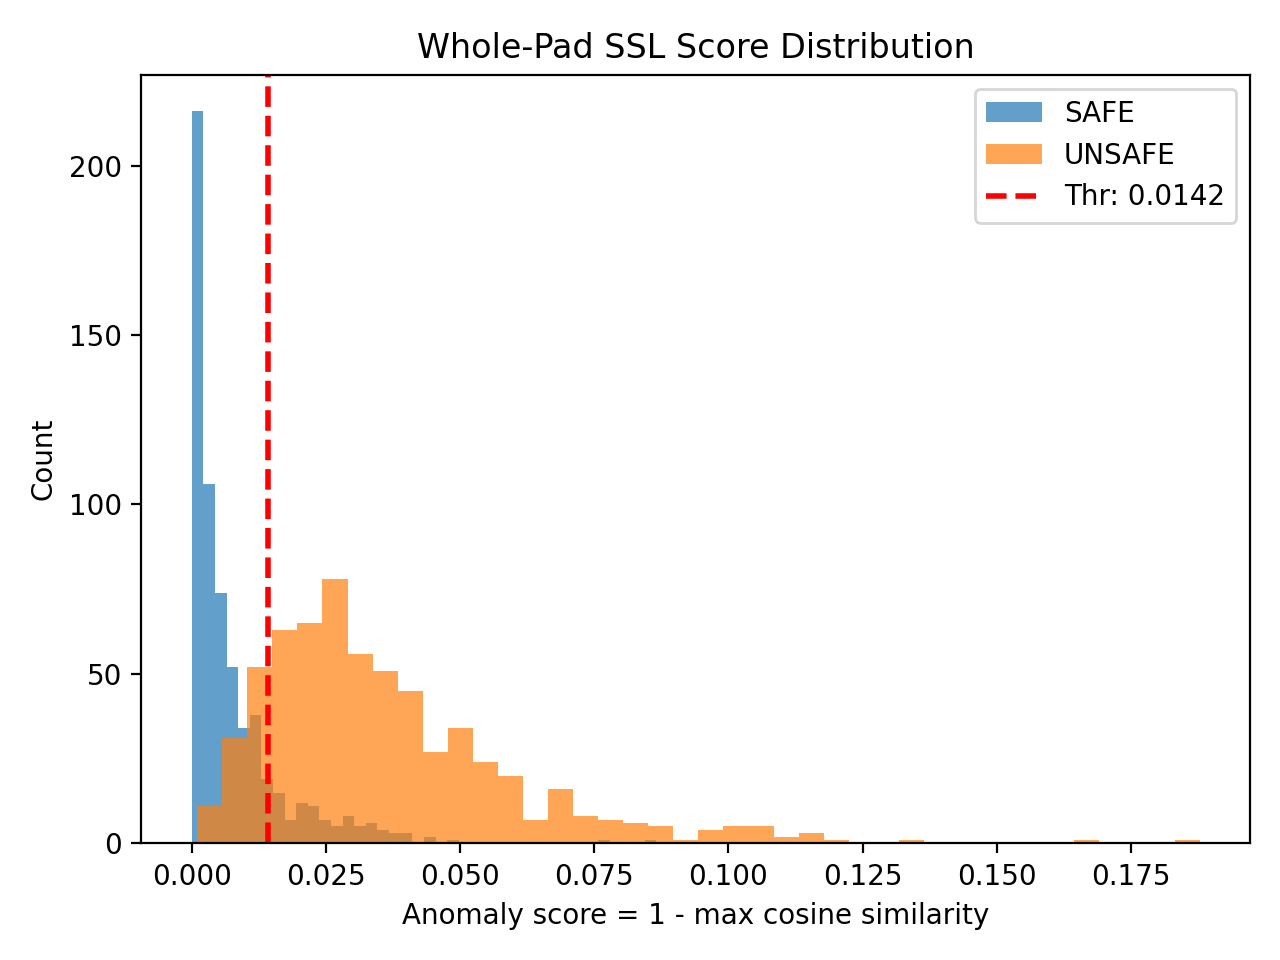
\includegraphics[width=0.47\textwidth]{figures/wholepad_hist.png}\hfill
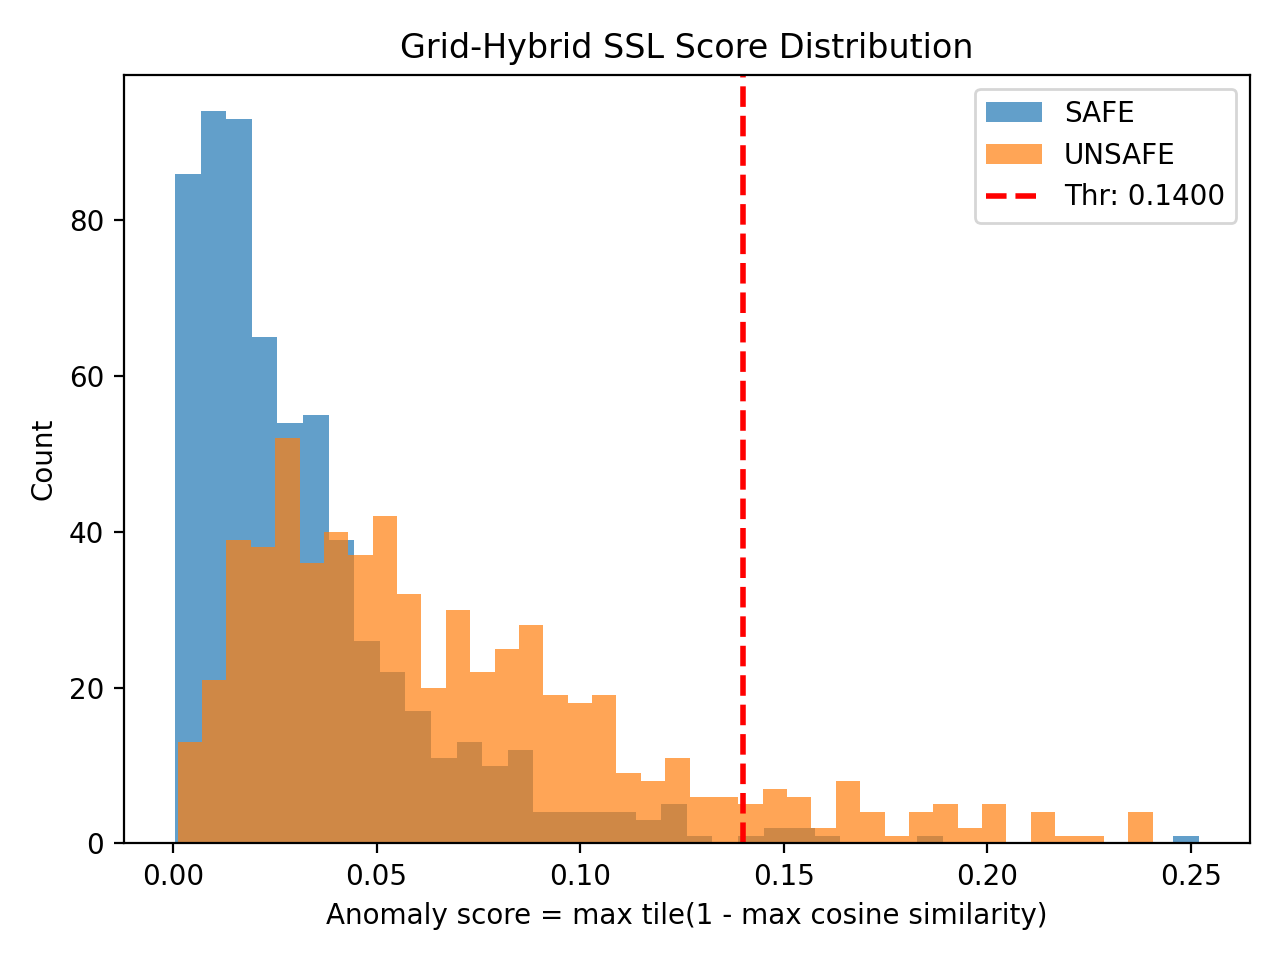
\includegraphics[width=0.47\textwidth]{figures/grid_hist.png}
\caption{Anomaly-score distributions and evaluated decision thresholds for Wholepad SSL (left) and Grid-Hybrid SSL (right).}
\label{fig:hist}
\end{figure*}

Grid-Hybrid is highly sensitive to calibration. Replacing its stored threshold with the Youden threshold, 0.03994, raises recall from 0.0921 to 0.6571 and F1 from 0.1667 to 0.6832, with specificity 0.7333. The best-F1 threshold on this evaluation set, 0.02190, yields 0.8603 recall and 0.7217 F1 but only 0.4762 specificity. These are diagnostic, post-hoc operating points rather than unbiased deployment estimates. Wholepad is more stable: its best-F1 threshold of 0.01166 produces 0.9111 recall and 0.8606 F1, close to its Youden-selected result.

\section{Discussion}
The global representation appears better matched to this synthetic protocol. The occlusions cover up to 65\% of a pad and deliberately introduce strong contrast, structured texture, contours, and shadows. Such changes alter the overall pad representation and are readily exposed by a nearest-neighbor comparison. The tiled model was designed to prevent small hazards from being diluted, yet its active threshold suppresses most positive decisions.

Representation granularity is not the only difference between the systems. Wholepad scoring uses 2,048-dimensional encoder features, whereas Grid-Hybrid uses 128-dimensional projector features; the latter also compares every quadrant against a position-pooled bank. A normal-looking tile from any quadrant can therefore provide a strong match, and the lower-dimensional projection may discard details useful for anomaly separation. Consequently, the experiment supports the complete Wholepad pipeline but does not isolate a causal advantage for global cropping alone. A controlled ablation should keep feature space, bank sampling, augmentation policy, and threshold calibration fixed.

The synthetic benchmark has four further limitations. First, procedural obstructions are conspicuous and do not cover all real hazards, including transparent materials, low-contrast debris, specular surfaces, or shadows without physical obstacles. Second, each anomalous sample shares its background with a clean sample, so confidence intervals must respect pairing. Third, the threshold fallback and post-hoc alternatives are computed on the evaluated scores; a separate calibration split is required for deployment. Fourth, the current results measure discrimination, not latency, memory transfer, or end-to-end landing risk.

Despite these constraints, the paired protocol is useful for controlled development. It exposes the effect of an obstruction without changing viewpoint or pad identity and reveals whether a model's score responds in the intended direction. Future work should validate on real, independently annotated pad hazards; calibrate thresholds on a held-out split; compare position-specific and coreset memory banks; and report resource use on the target UAV computer.

\section{Conclusion}
This study evaluated two self-supervised, memory-bank anomaly detectors for UAV landing pads using reproducible synthetic occlusions. Under a balanced 1,260-sample paired test, Wholepad SSL achieved 0.9236 AUROC and balanced precision-recall behavior, while Grid-Hybrid SSL reached 0.7555 AUROC and suffered severe false negatives at its stored threshold. The results favor the complete Wholepad pipeline for the tested obstruction family and show that threshold calibration can materially change the apparent safety profile of the tiled model. Real-hazard validation and controlled representation ablations remain necessary before flight deployment.

\begin{thebibliography}{00}
\bibitem{chen2020} T. Chen, S. Kornblith, M. Norouzi, and G. Hinton, "A simple framework for contrastive learning of visual representations," in \emph{Proc. ICML}, 2020, pp. 1597--1607.
\bibitem{roth2022} K. Roth, L. Pemula, J. Zepeda, B. Sch\"olkopf, T. Brox, and P. Gehler, "Towards total recall in industrial anomaly detection," in \emph{Proc. IEEE/CVF CVPR}, 2022, pp. 14318--14328.
\bibitem{he2016} K. He, X. Zhang, S. Ren, and J. Sun, "Deep residual learning for image recognition," in \emph{Proc. IEEE CVPR}, 2016, pp. 770--778.
\bibitem{redmon2016} J. Redmon, S. Divvala, R. Girshick, and A. Farhadi, "You only look once: Unified, real-time object detection," in \emph{Proc. IEEE CVPR}, 2016, pp. 779--788.
\bibitem{defard2021} T. Defard, A. Setkov, A. Loesch, and R. Audigier, "PaDiM: A patch distribution modeling framework for anomaly detection and localization," in \emph{Pattern Recognition: ICPR International Workshops and Challenges}. Springer, 2021, pp. 475--489.
\bibitem{cohen2020} N. Cohen and Y. Hoshen, "Sub-image anomaly detection with deep pyramid correspondences," in \emph{Proc. ICML}, 2020, pp. 2058--2067.
\bibitem{tack2020} J. Tack, S. Mo, J. Jeong, and J. Shin, "CSI: Novelty detection via contrastive learning on distributionally shifted instances," in \emph{NeurIPS}, vol. 33, 2020, pp. 11839--11852.
\bibitem{ruff2021} L. Ruff \emph{et al.}, "A unifying review of deep and shallow anomaly detection," \emph{Proc. IEEE}, vol. 109, no. 5, pp. 756--795, 2021.
\bibitem{reiss2021} T. Reiss, N. Cohen, L. Bergman, and Y. Hoshen, "PANDA: Adapting pretrained features for anomaly detection and segmentation," in \emph{Proc. IEEE/CVF CVPR}, 2021, pp. 2806--2814.
\bibitem{yang2013} S. Yang, S. A. Scherer, and A. Zell, "An onboard visual autonomous landing system for quadrotors in GPS-denied environments," in \emph{Proc. IEEE ICRA}, 2013, pp. 2736--2741.
\bibitem{abdollahzadeh2026} S. Abdollahzadeh, M. S. Allili, A. Boulmerka, and J.-F. Lapointe, "A vision-based framework for safe landing zone mapping of UAVs in dynamic environments," \emph{IEEE Open J. Comput. Soc.}, 2026, doi: 10.1109/OJCS.2026.3663268.
\bibitem{hojjati2022} H. Hojjati, T. K. K. Ho, and N. Armanfard, "Self-supervised anomaly detection in computer vision and beyond: A survey and outlook," arXiv:2205.05173, 2022.
\bibitem{akram2024} J. Akram, A. Anaissi, W. Othman, A. Alabdulatif, and A. Akram, "DroneSSL: Self-supervised multimodal anomaly detection in Internet of Drone Things," \emph{IEEE Trans. Consum. Electron.}, vol. 70, no. 1, pp. 4287--4298, 2024.
\bibitem{teknofest2026} TEKNOFEST, "Havacilikta Yapay Zeka Yarismasi 2026 data set," 2026. [Online]. Available: \url{https://drive.google.com/drive/folders/18_VqLBbyTubVSWAXG_CgmuJWGCx0mcBd}
\end{thebibliography}

\end{document}

